\section{包设计}
\section{具体功能设计}
\subsection{注册登录模块}
\subsubsection{模块内部接口}
\begin{figure}[!htb]
	\centering
	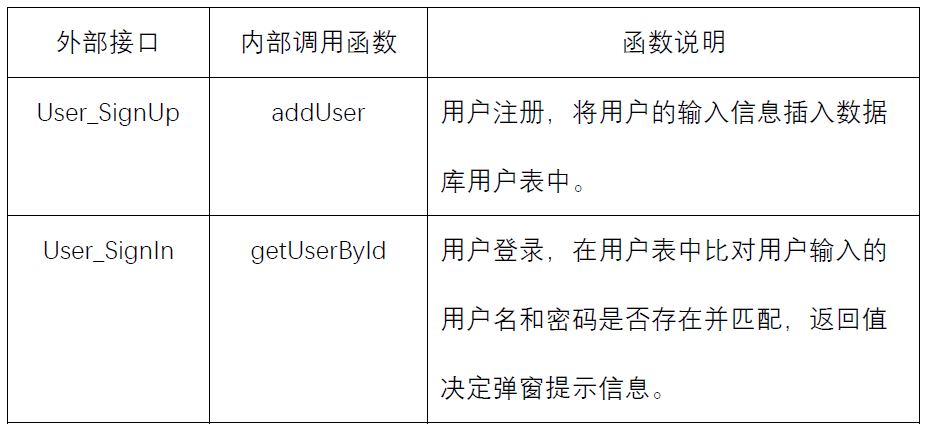
\includegraphics[scale=1]{image/b1.png} %修改路径下图片名称 scale 图片缩放
	\caption{table1} %修改图例(图片标题)
\end{figure}
\subsubsection{内部接口设计}
\subsubsubsection{注册实现接口}
\begin{figure}[!htb]
	\centering
	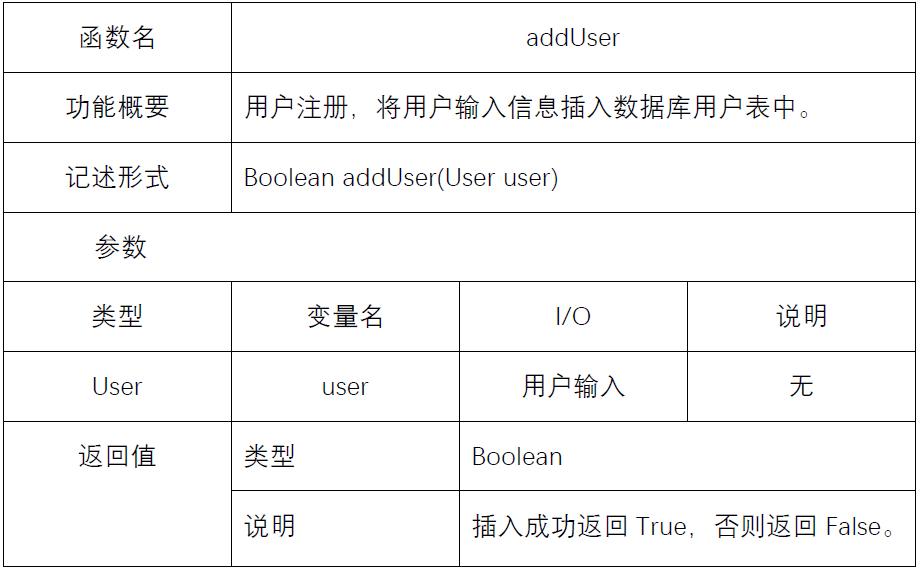
\includegraphics[scale=1]{image/b2.png} %修改路径下图片名称 scale 图片缩放
	\caption{table2} %修改图例(图片标题)
\end{figure}
\subsubsubsection{登录实现接口}
\begin{figure}[!htb]
	\centering
	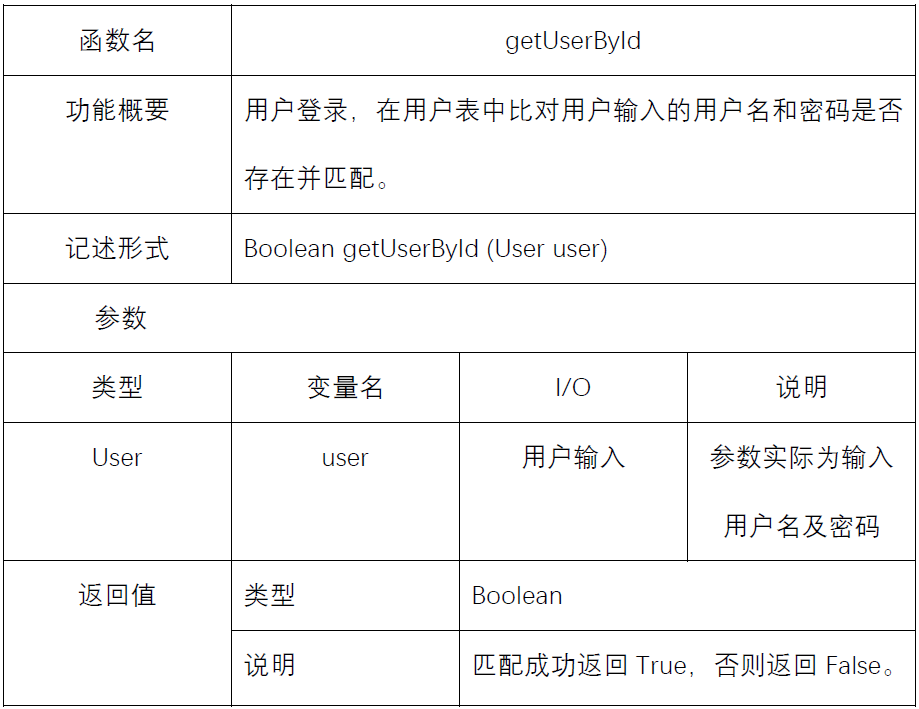
\includegraphics[scale=1]{image/b3.png} %修改路径下图片名称 scale 图片缩放
	\caption{table3} %修改图例(图片标题)
\end{figure}
\subsection{搜索模块}
\subsubsection{模块内部接口}
\begin{figure}[!htb]
	\centering
	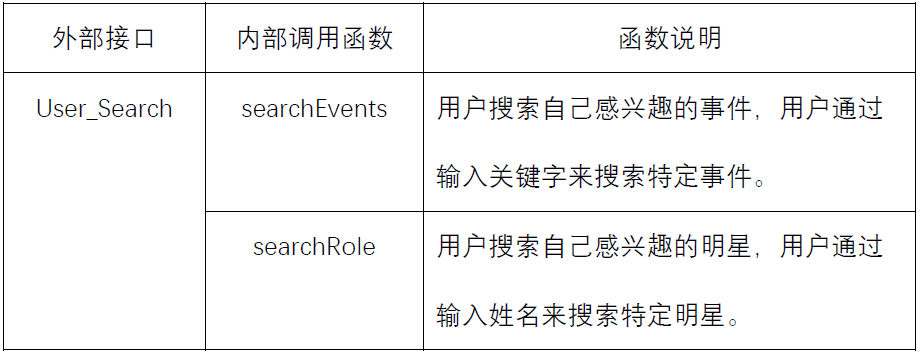
\includegraphics[scale=1]{image/b4.png} %修改路径下图片名称 scale 图片缩放
	\caption{table4} %修改图例(图片标题)
\end{figure}
\subsubsection{内部接口设计}
\subsubsubsection{搜索热点事件}
\begin{figure}[!htb]
	\centering
	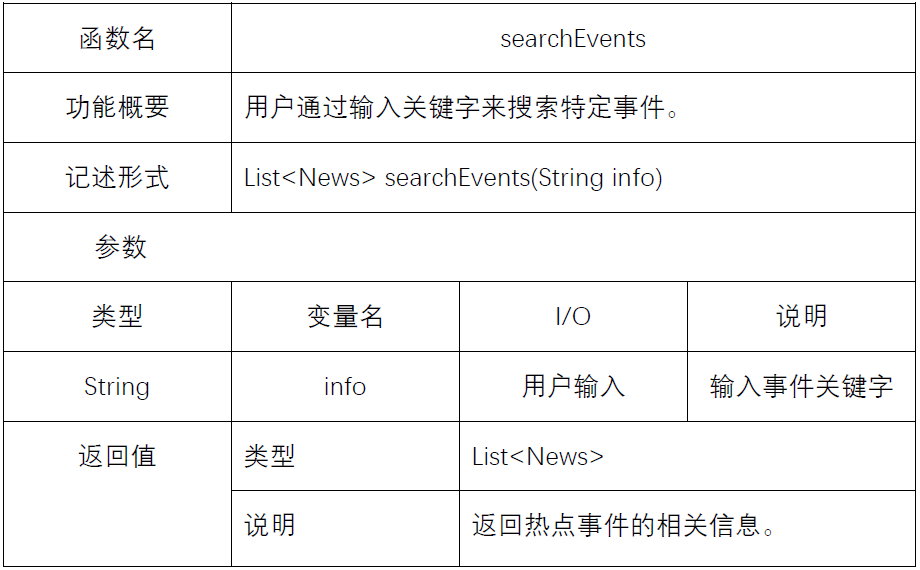
\includegraphics[scale=1]{image/b5.png} %修改路径下图片名称 scale 图片缩放
	\caption{table5} %修改图例(图片标题)
\end{figure}
\subsubsubsection{搜索热点明星}
\begin{figure}[!htb]
	\centering
	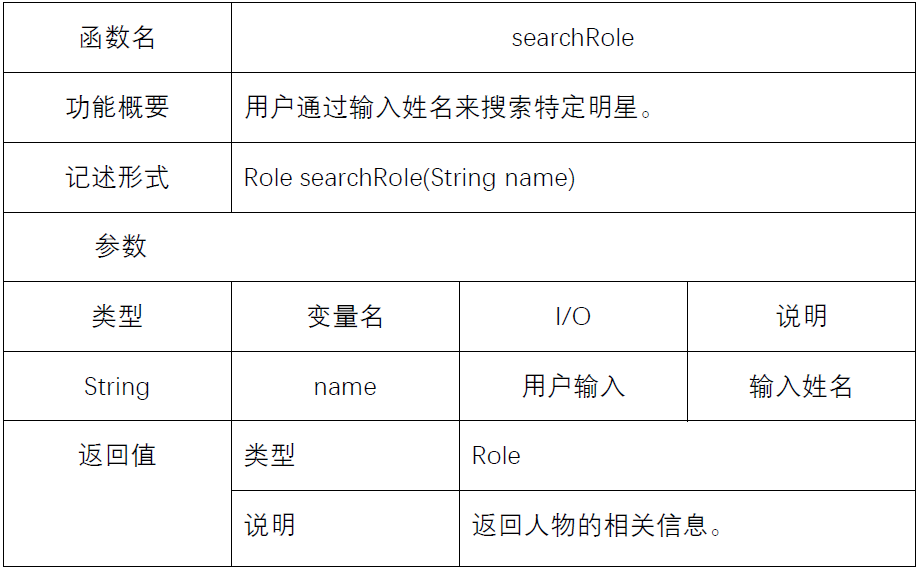
\includegraphics[scale=1]{image/b6.png} %修改路径下图片名称 scale 图片缩放
	\caption{table6} %修改图例(图片标题)
\end{figure}
\subsection{展示模块}
\subsubsection{模块内部接口}
\begin{figure}[!htb]
	\centering
	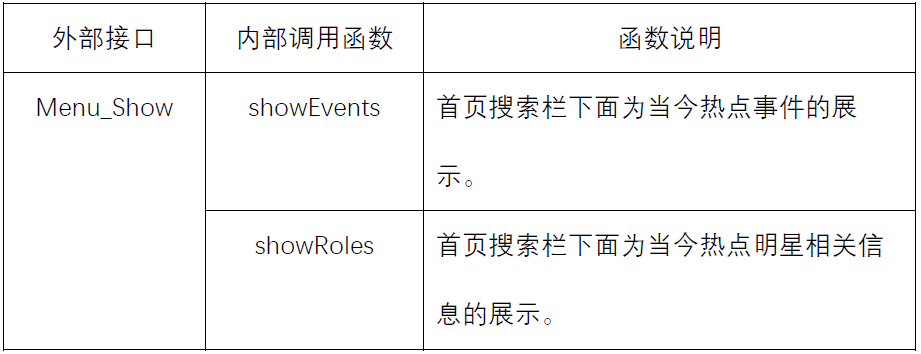
\includegraphics[scale=1]{image/b7.png} %修改路径下图片名称 scale 图片缩放
	\caption{table7} %修改图例(图片标题)
\end{figure}
\subsubsection{内部接口设计}
\subsubsubsection{展示热点事件}
\begin{figure}[!htb]
	\centering
	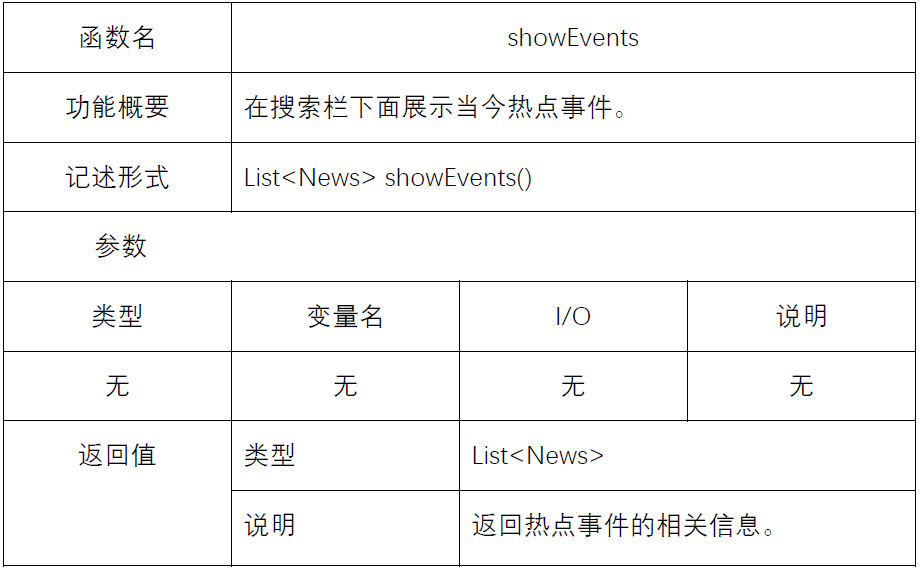
\includegraphics[scale=1]{image/b8.png} %修改路径下图片名称 scale 图片缩放
	\caption{table8} %修改图例(图片标题)
\end{figure}
\subsubsubsection{展示热点明星}
\begin{figure}[!htb]
	\centering
	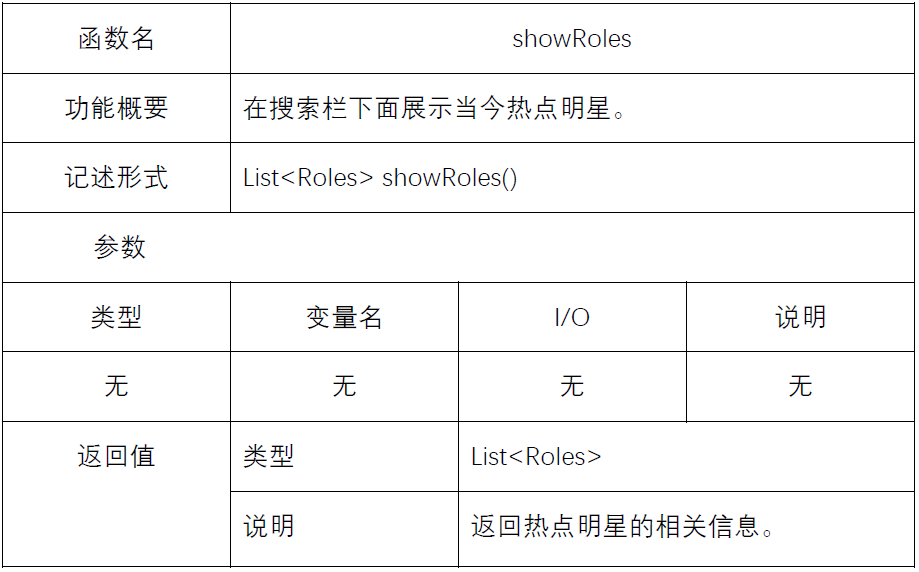
\includegraphics[scale=1]{image/b9.png} %修改路径下图片名称 scale 图片缩放
	\caption{table9} %修改图例(图片标题)
\end{figure}
\subsection{记录查询模块}
\subsubsection{模块内部接口}
\begin{figure}[!htb]
	\centering
	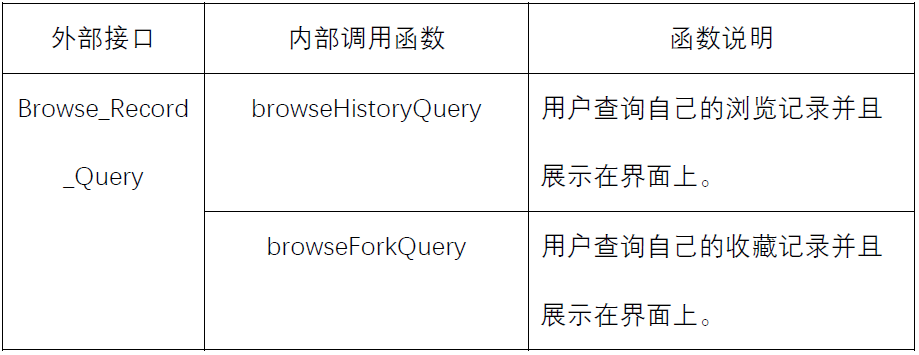
\includegraphics[scale=1]{image/b10.png} %修改路径下图片名称 scale 图片缩放
	\caption{table10} %修改图例(图片标题)
\end{figure}
\subsubsection{内部接口设计}
\subsubsubsection{查询浏览记录}
\begin{figure}[!htb]
	\centering
	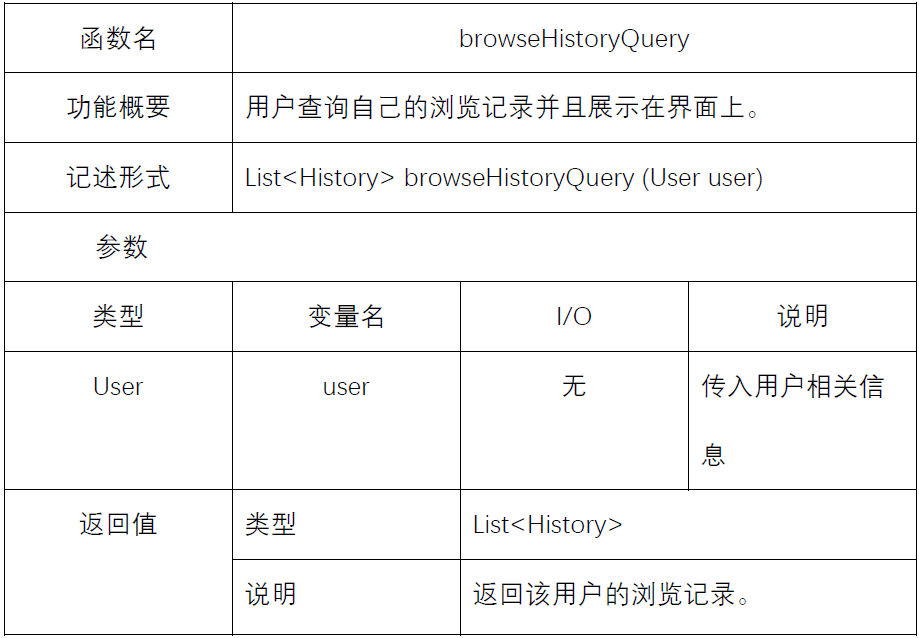
\includegraphics[scale=1]{image/b11.png} %修改路径下图片名称 scale 图片缩放
	\caption{table11} %修改图例(图片标题)
\end{figure}
\subsubsubsection{查询收藏记录}
\begin{figure}[!htb]
	\centering
	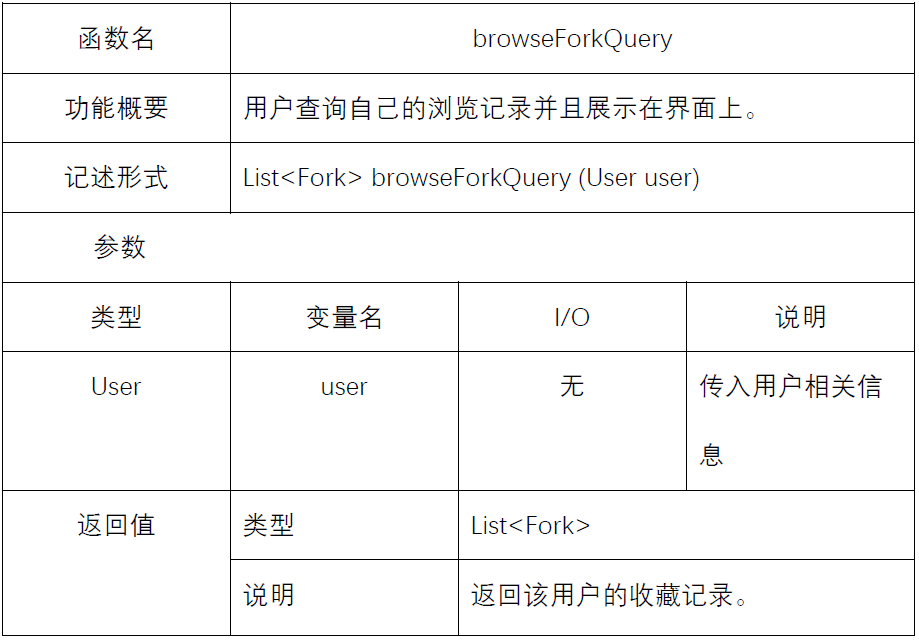
\includegraphics[scale=1]{image/b12.png} %修改路径下图片名称 scale 图片缩放
	\caption{table12} %修改图例(图片标题)
\end{figure}
\subsection{支付模块}
\subsubsection{模块内部接口}
\begin{figure}[!htb]
	\centering
	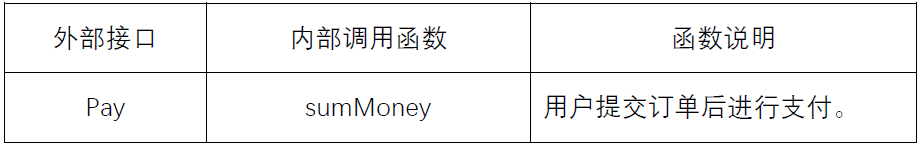
\includegraphics[scale=1]{image/b13.png} %修改路径下图片名称 scale 图片缩放
	\caption{table13} %修改图例(图片标题)
\end{figure}
\subsubsection{内部接口设计}
\subsubsubsection{支付功能}
\begin{figure}[!htb]
	\centering
	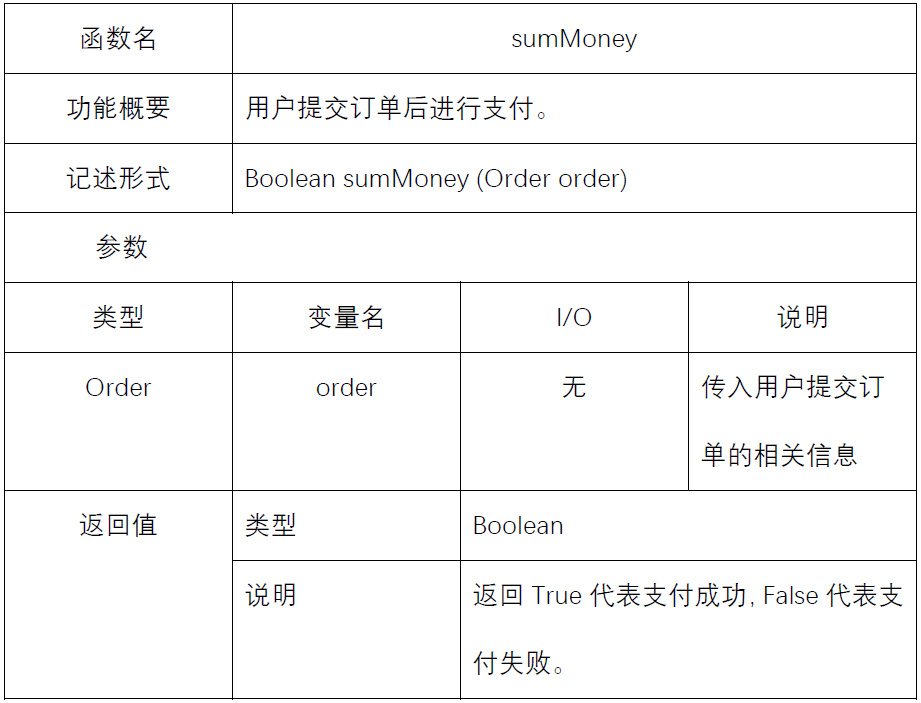
\includegraphics[scale=1]{image/b14.png} %修改路径下图片名称 scale 图片缩放
	\caption{table14} %修改图例(图片标题)
\end{figure}
\subsection{监控预警模块}
\subsubsection{模块内部接口}
\begin{figure}[!htb]
	\centering
	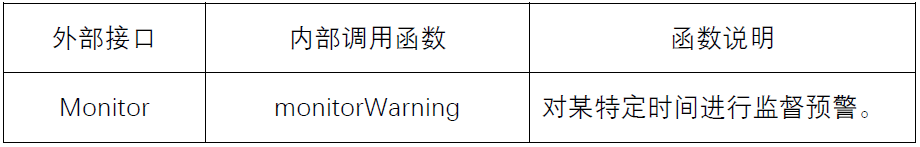
\includegraphics[scale=1]{image/b15.png} %修改路径下图片名称 scale 图片缩放
	\caption{table15} %修改图例(图片标题)
\end{figure}
\subsubsection{内部接口设计}
\subsubsubsection{监控预警功能}
\begin{figure}[!htb]
	\centering
	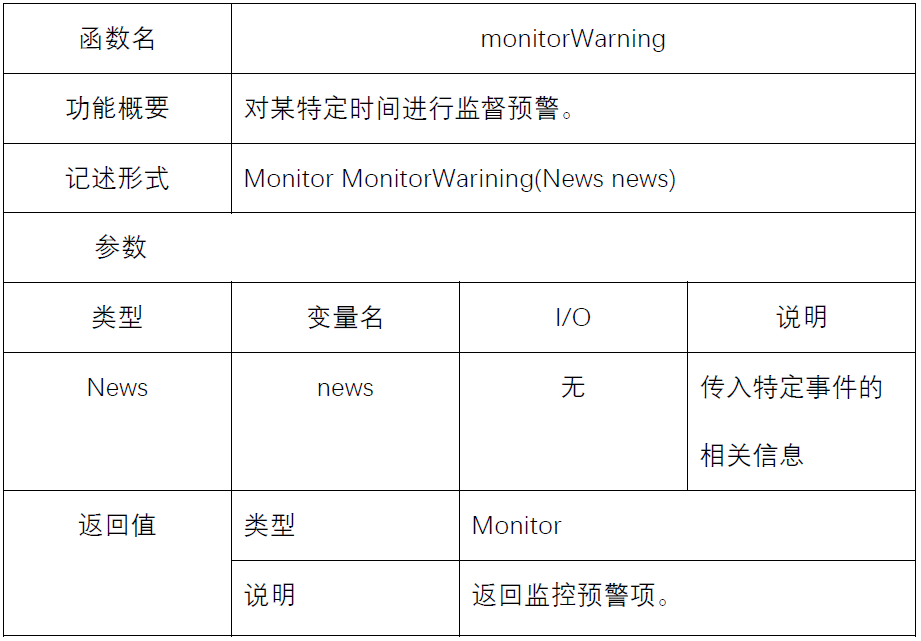
\includegraphics[scale=1]{image/b16.png} %修改路径下图片名称 scale 图片缩放
	\caption{table16} %修改图例(图片标题)
\end{figure}
\subsection{排行榜功能}
\subsubsection{模块内部接口}
\begin{figure}[!htb]
	\centering
	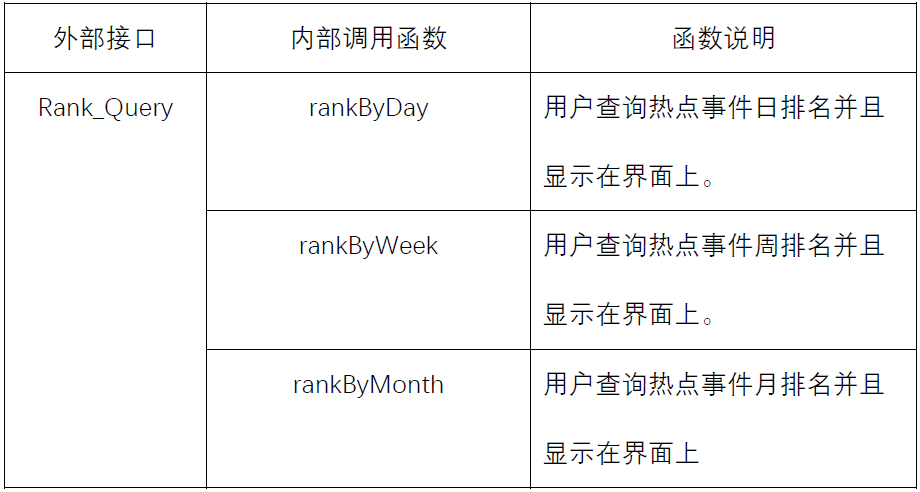
\includegraphics[scale=1]{image/b17.png} %修改路径下图片名称 scale 图片缩放
	\caption{table17} %修改图例(图片标题)
\end{figure}
\subsubsection{内部接口设计}
\subsubsubsection{查询日排名}
\begin{figure}[!htb]
	\centering
	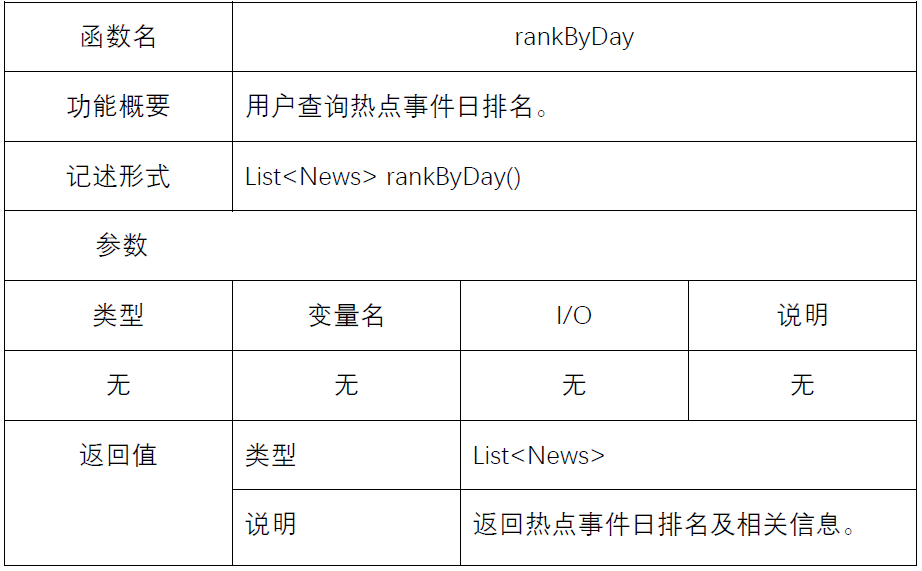
\includegraphics[scale=1]{image/b18.png} %修改路径下图片名称 scale 图片缩放
	\caption{table18} %修改图例(图片标题)
\end{figure}
\subsubsubsection{查询周排名}
\begin{figure}[!htb]
	\centering
	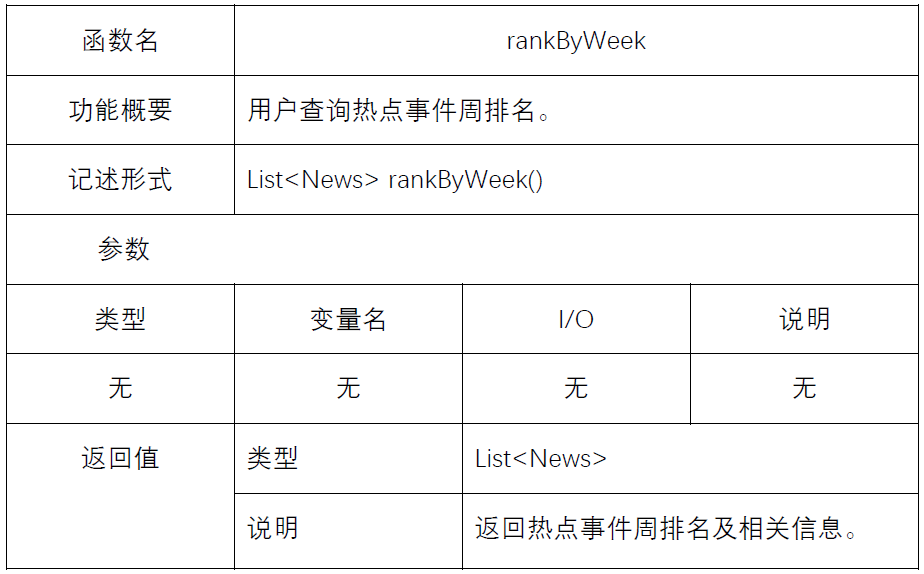
\includegraphics[scale=1]{image/b19.png} %修改路径下图片名称 scale 图片缩放
	\caption{table19} %修改图例(图片标题)
\end{figure}
\subsubsubsection{查询月排名}
\begin{figure}[!htb]
	\centering
	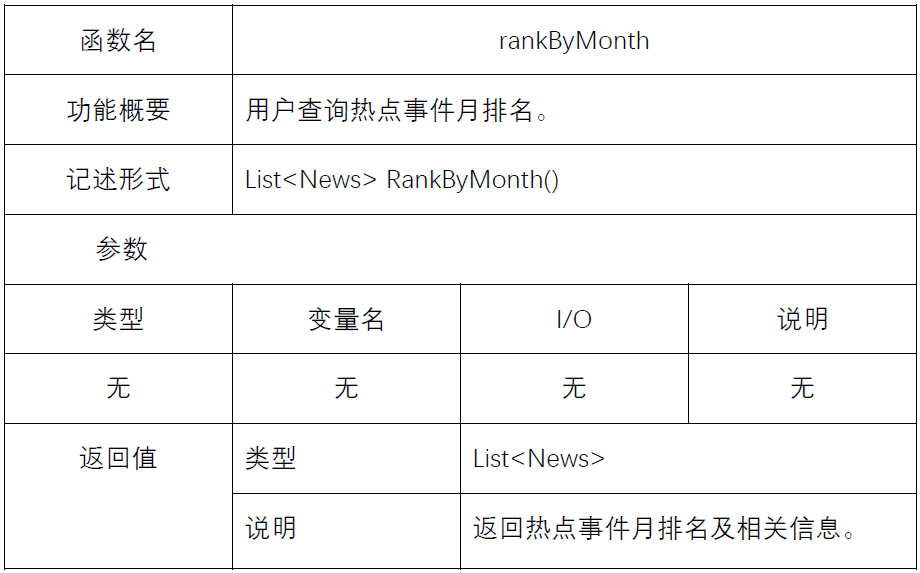
\includegraphics[scale=1]{image/b20.png} %修改路径下图片名称 scale 图片缩放
	\caption{table20} %修改图例(图片标题)
\end{figure}
\subsection{分析模块}
\subsubsection{模块内部接口}
\begin{figure}[!htb]
	\centering
	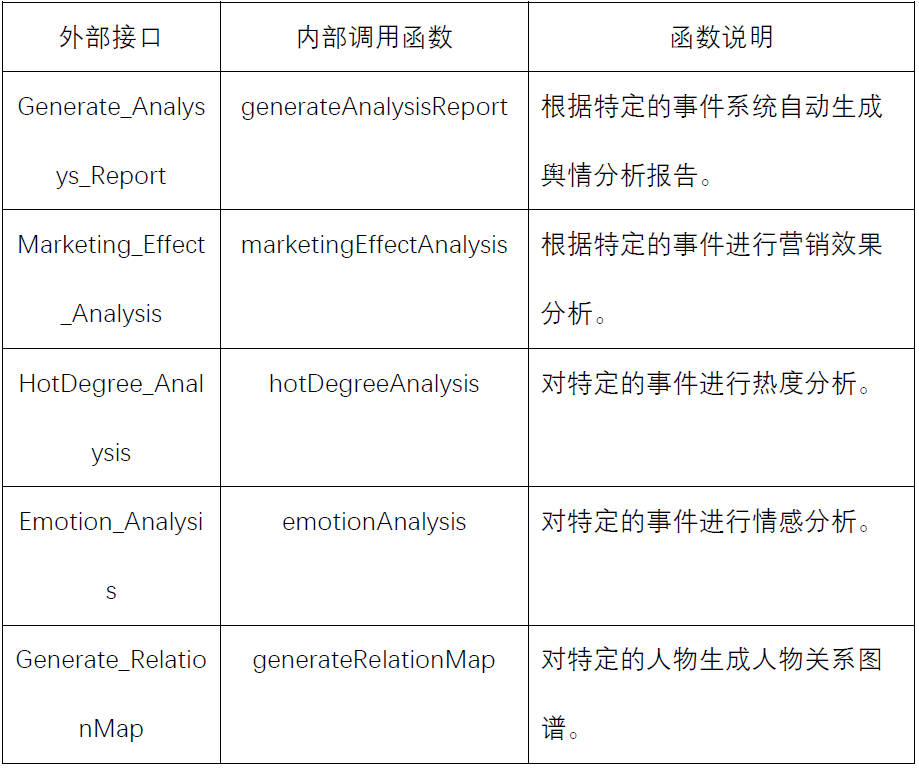
\includegraphics[scale=1]{image/b21.png} %修改路径下图片名称 scale 图片缩放
	\caption{table21} %修改图例(图片标题)
\end{figure}
\subsubsection{内部接口设计}
\subsubsubsection{生成分析报告功能}
\begin{figure}[!htb]
	\centering
	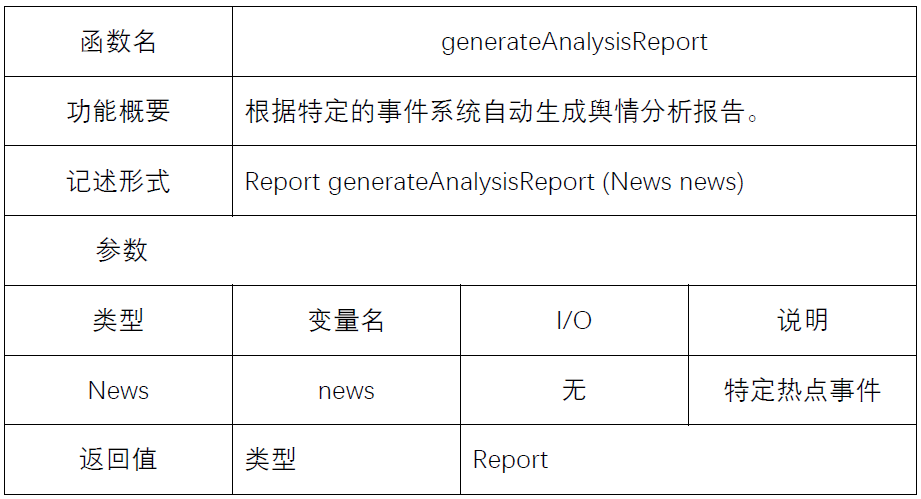
\includegraphics[scale=1]{image/b22.png} %修改路径下图片名称 scale 图片缩放
	\caption{table22} %修改图例(图片标题)
\end{figure}
\begin{figure}[!htb]
	\centering
	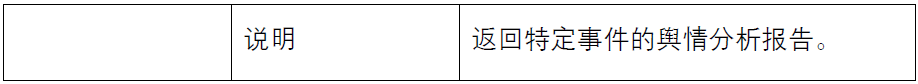
\includegraphics[scale=1]{image/b27.png} %修改路径下图片名称 scale 图片缩放
	\caption{table27} %修改图例(图片标题)
\end{figure}
\subsubsubsection{营销效果分析功能}
\begin{figure}[!htb]
	\centering
	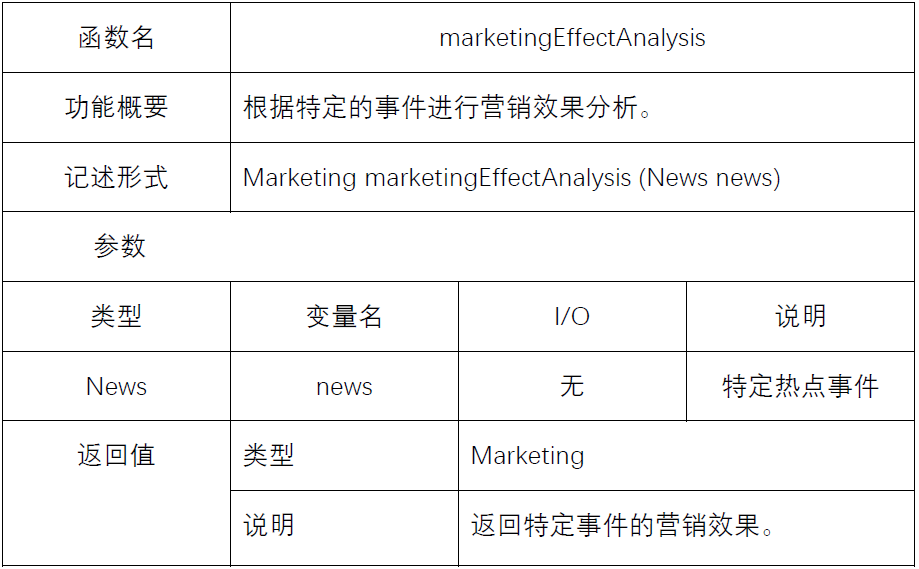
\includegraphics[scale=1]{image/b23.png} %修改路径下图片名称 scale 图片缩放
	\caption{table23} %修改图例(图片标题)
\end{figure}
\subsubsubsection{热度分析功能}
\begin{figure}[!htb]
	\centering
	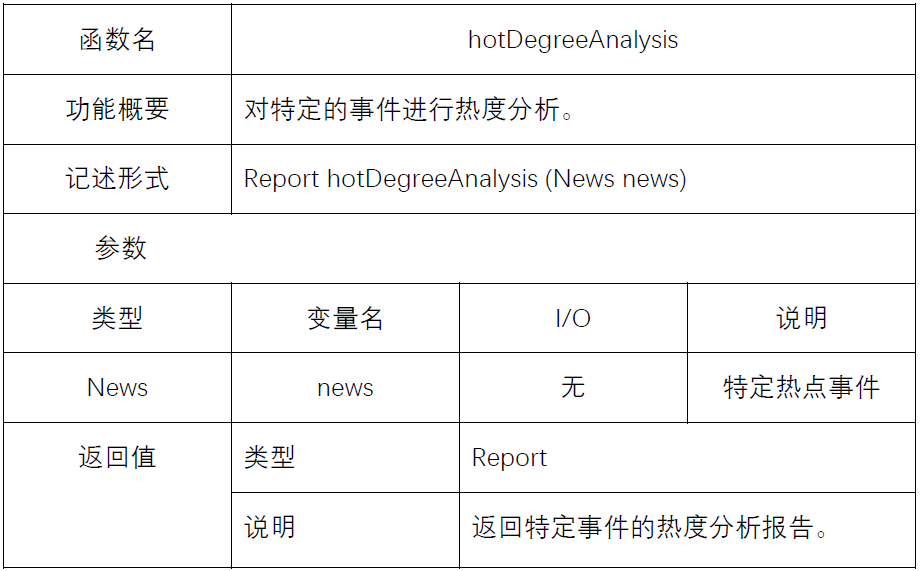
\includegraphics[scale=1]{image/b24.png} %修改路径下图片名称 scale 图片缩放
	\caption{table24} %修改图例(图片标题)
\end{figure}
\subsubsubsection{情感分析功能}
\begin{figure}[!htb]
	\centering
	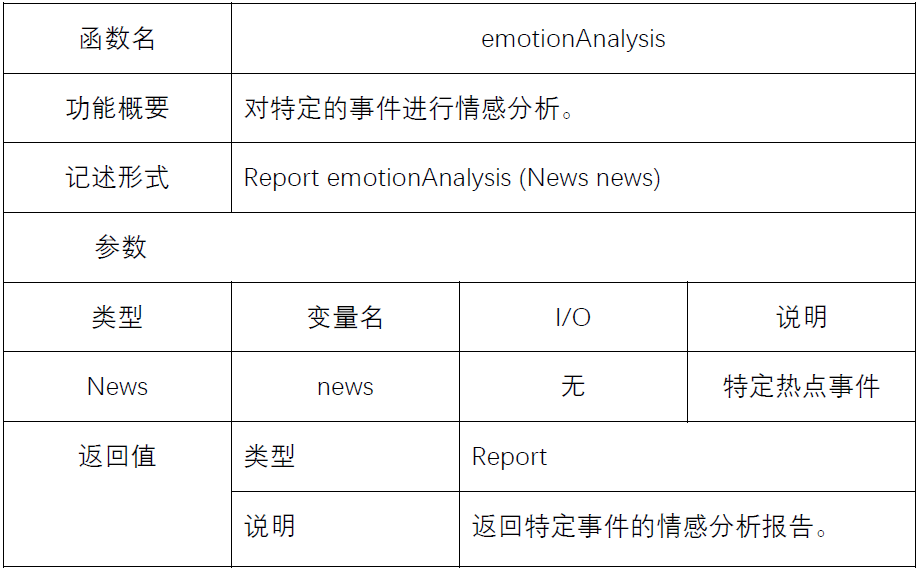
\includegraphics[scale=1]{image/b25.png} %修改路径下图片名称 scale 图片缩放
	\caption{table23} %修改图例(图片标题)
\end{figure}
\subsubsubsection{人物关系图谱功能}
\begin{figure}[!htb]
	\centering
	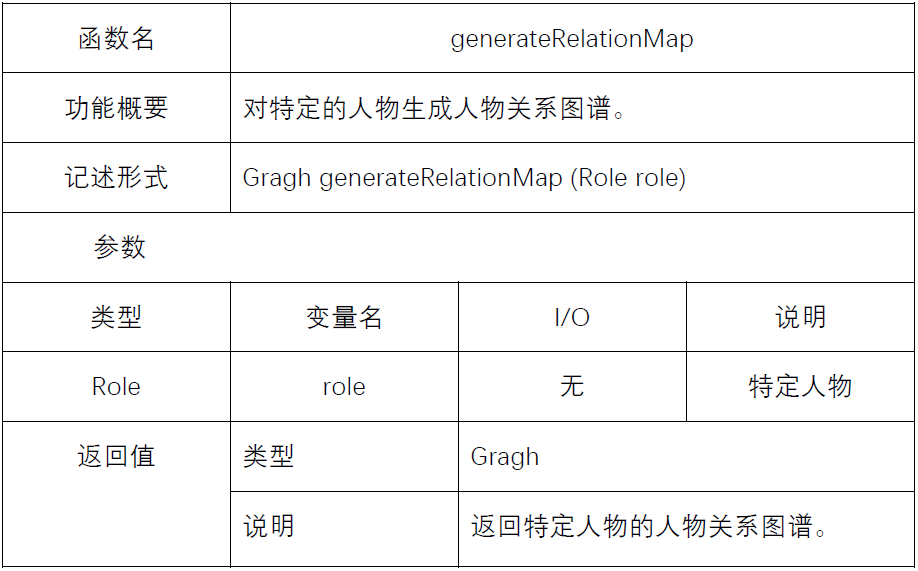
\includegraphics[scale=1]{image/b26.png} %修改路径下图片名称 scale 图片缩放
	\caption{table24} %修改图例(图片标题)
\end{figure}
